\begin{figure}[h!]
\begin{subfigure}
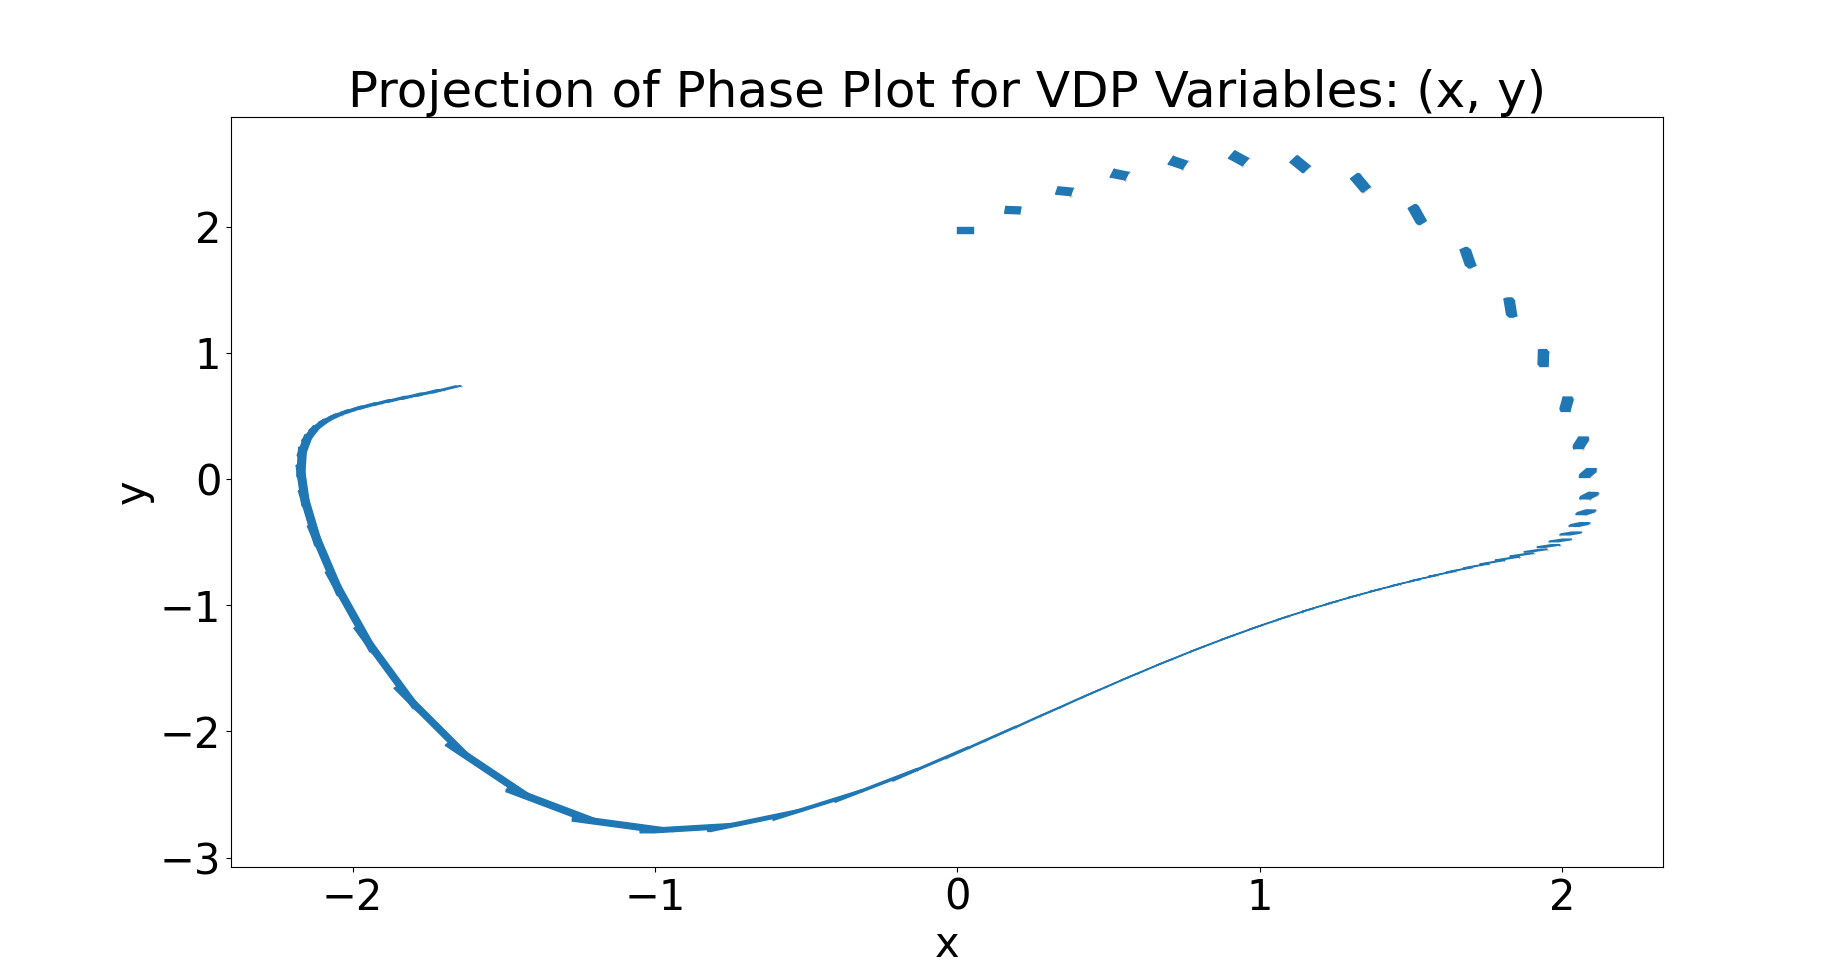
\includegraphics[width=\textwidth]{figures/PhasePlots/VDP_5Lin_.png}
\caption{5 Lin}
\end{subfigure}%
\begin{subfigure}
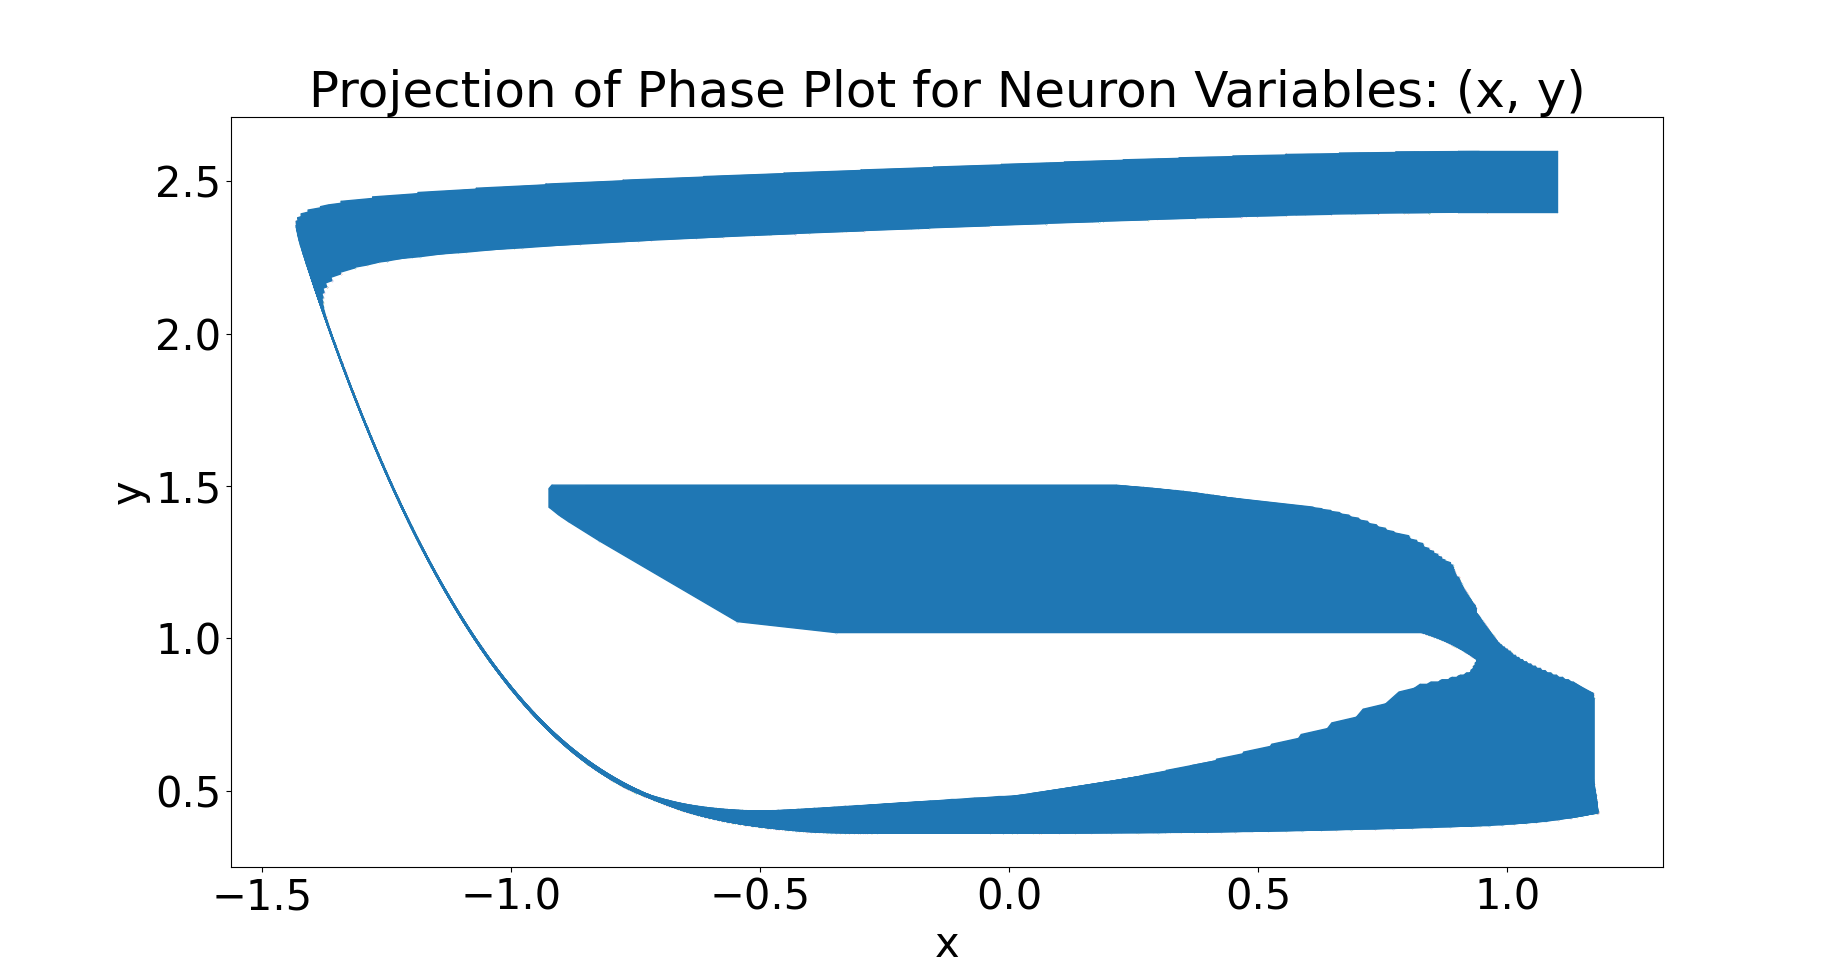
\includegraphics[width=\textwidth]{figures/PhasePlots/Neuron_1PCA5Lin_.png}
\caption{1 PCA 5 Lin}
\end{subfigure}%

\begin{subfigure}
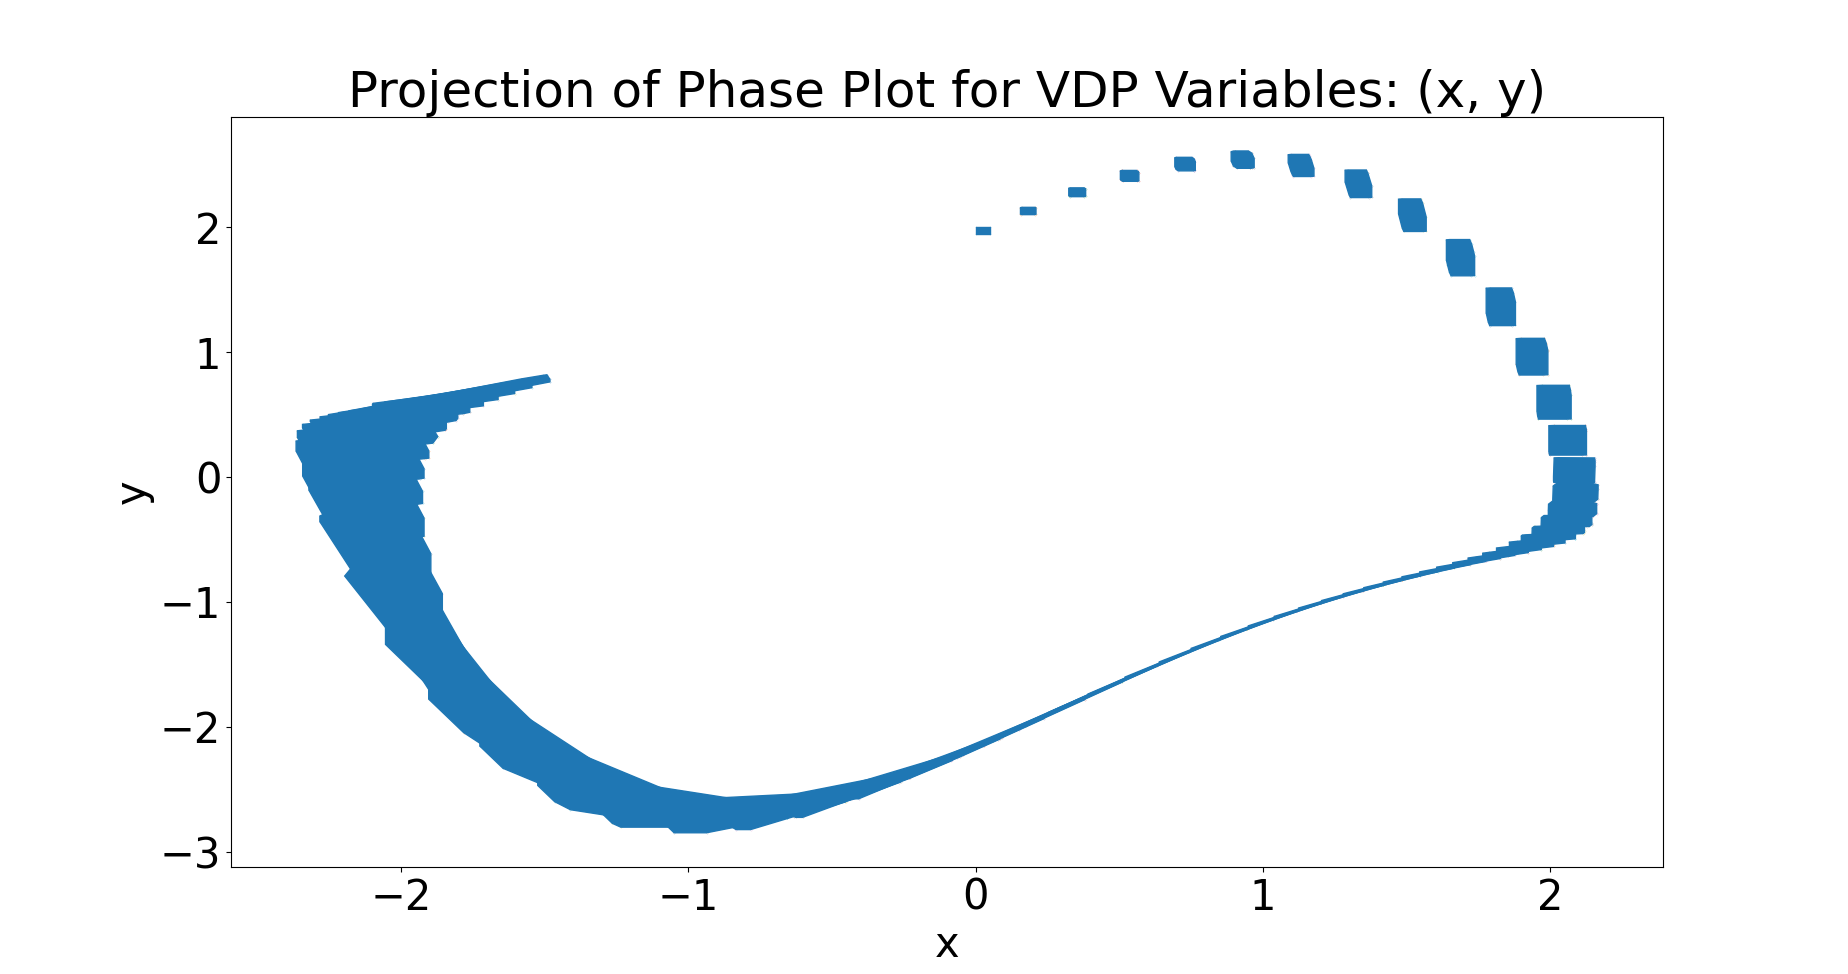
\includegraphics[width=\textwidth]{figures/PhasePlots/VDP_5PCA_.png}
\caption{5 PCA}
\end{subfigure}%
\begin{subfigure}
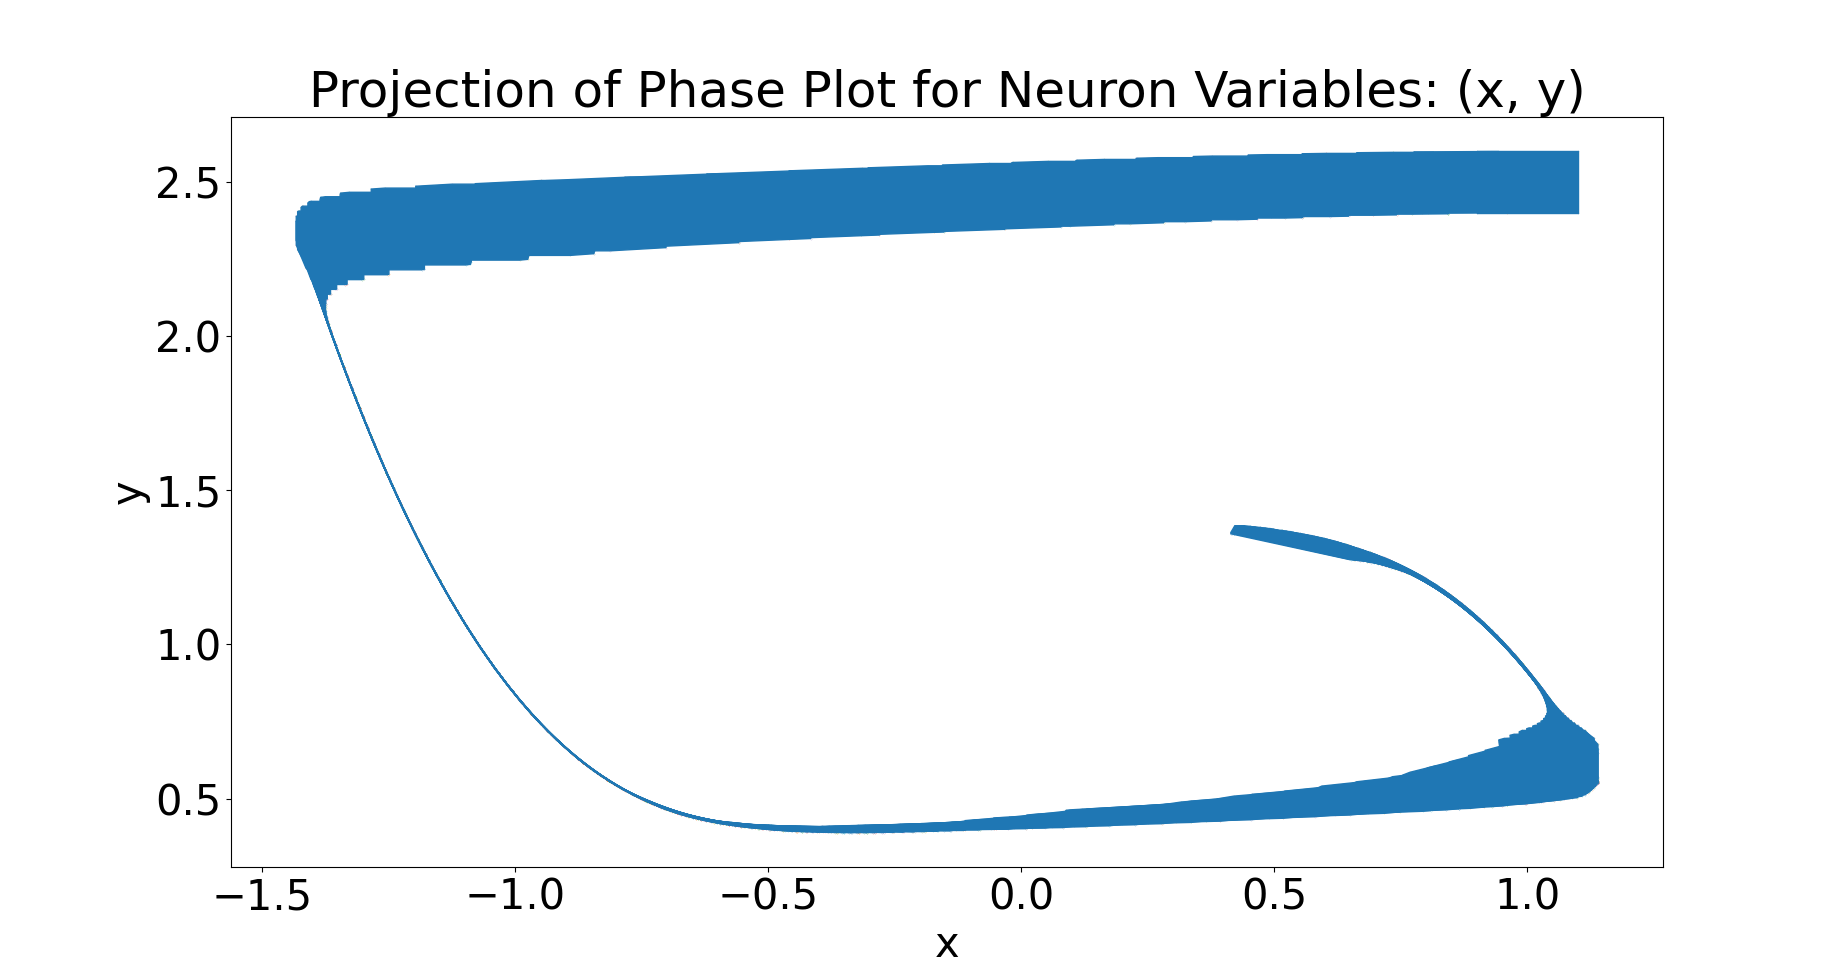
\includegraphics[width=\textwidth]{figures/PhasePlots/Neuron_5PCA1Lin_.png}
\caption{5 PCA 1 Lin}
\end{subfigure}

\begin{subfigure}
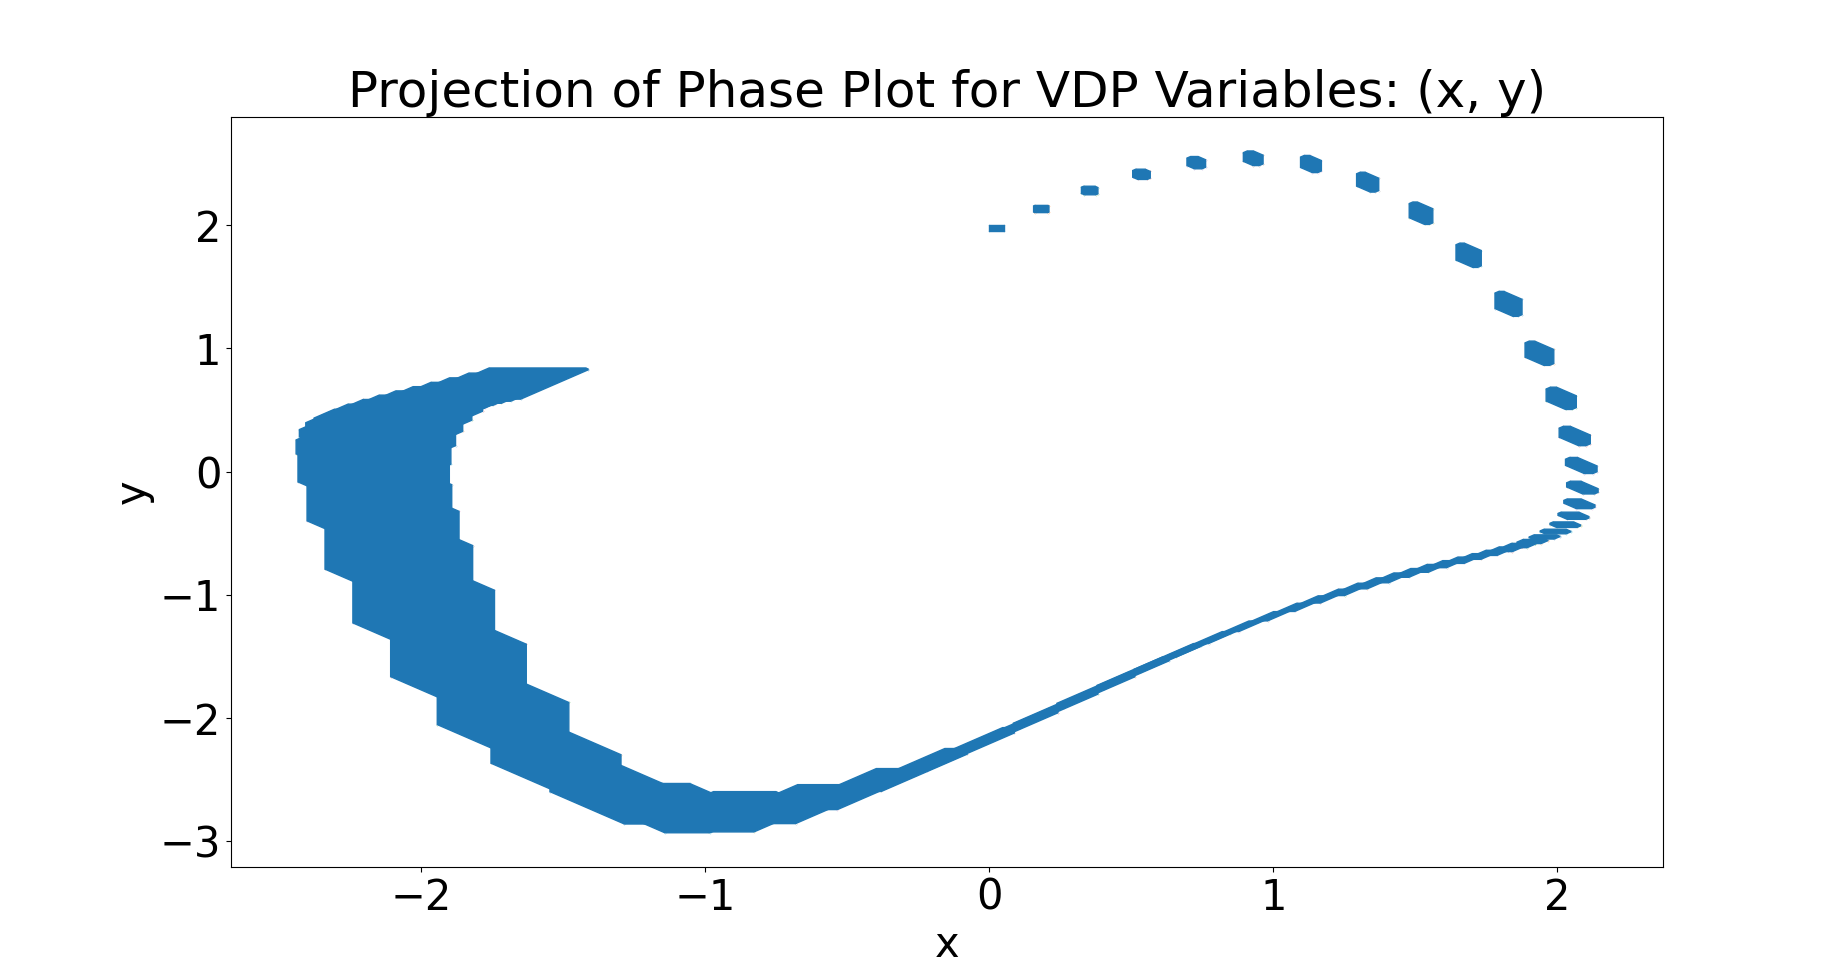
\includegraphics[width=\textwidth]{figures/PhasePlots/VDP_Sapo_.png}
\caption{Sapo}
\end{subfigure}%
\begin{subfigure}
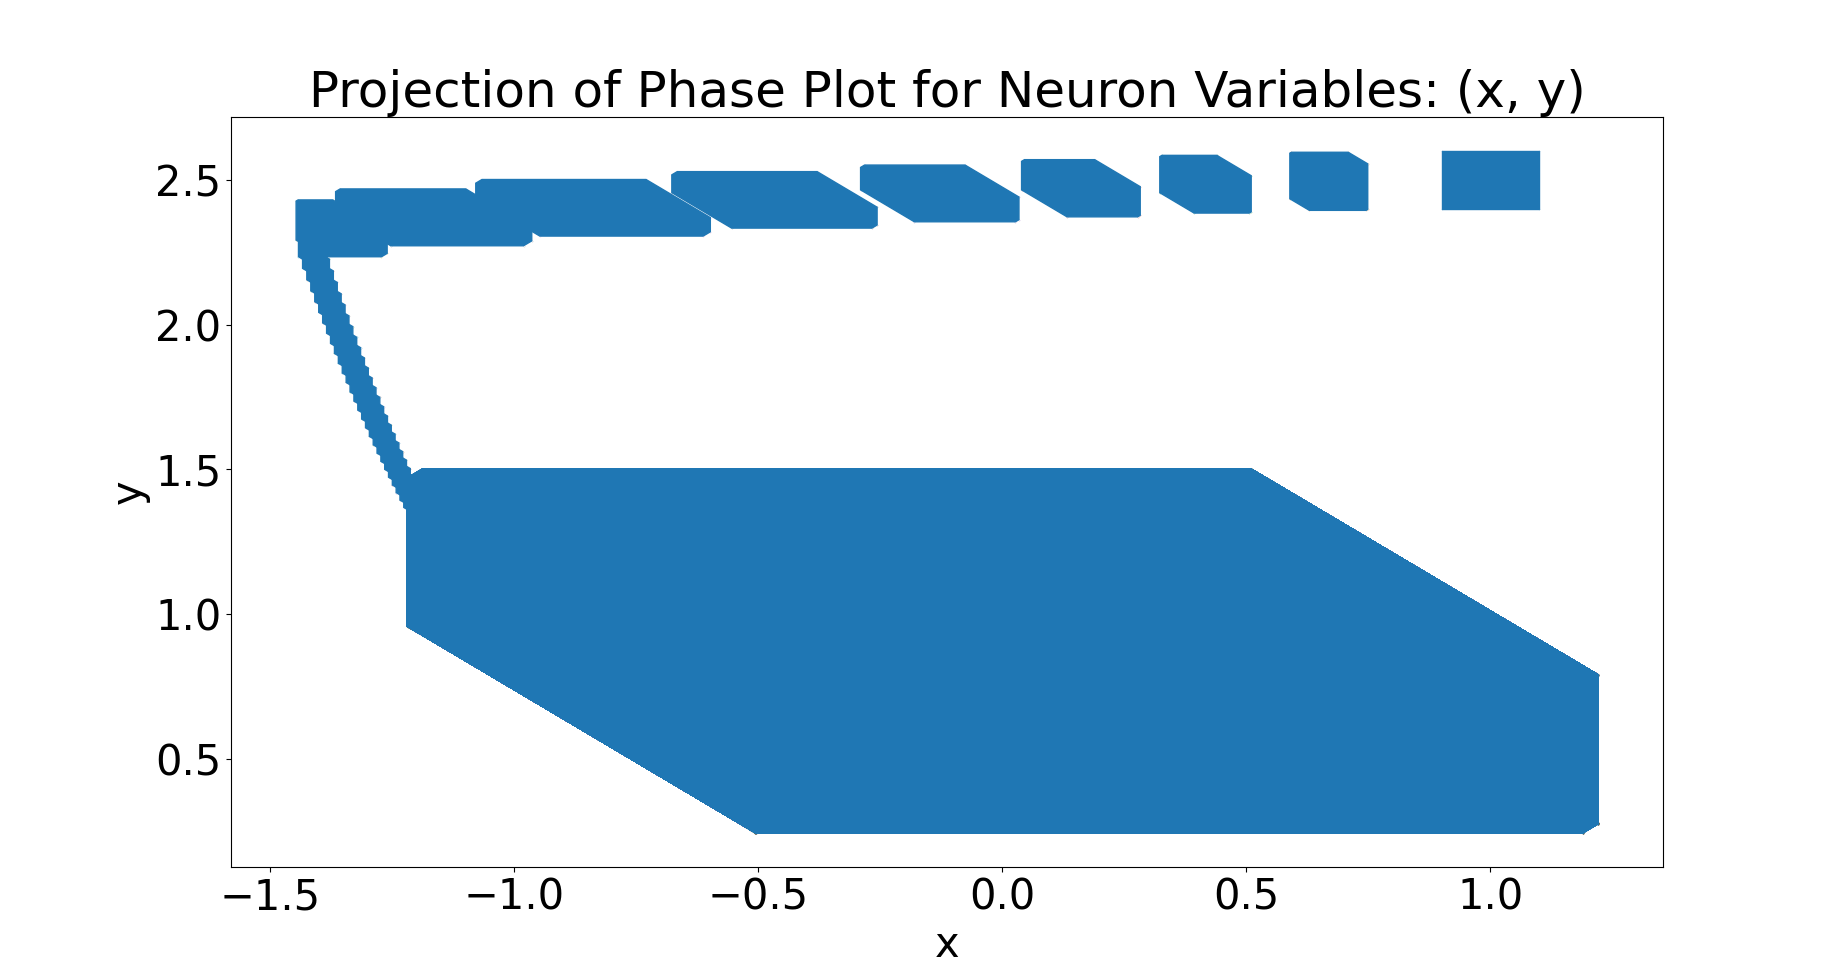
\includegraphics[width=\textwidth]{figures/PhasePlots/Neuron_Sapo_.png}
\caption{Sapo}
\end{subfigure}
\caption{Effect of varying ratio between the number of PCA and Linear Approximation parallelotopes. The Vanderpol (left) and the FitzHugh-Nagumo Neuron (right) phase plots are shown to illustrate differing effects of varying the PCA/LinApp ratio. The initial set for the Vanderpol model is set to $x \in [0,0.05], \, y \in [1.95,2]$}
\label{fig:PCALinAppRatio}
\end{figure}
